\section{Problem Description}
In order to realize a directional low-mid emission with three near-omnidirectional speakers, signal parameters have to be chosen in a specific manner. The directional characteristics of the speaker array depend on the amplitude and phase of the signal that is transduced via the individual speakers. The resulting directional characteristics of a given set of signal-parameters can be described by the use of an analytical model, that has been supplemented with knowledge from measuring the polar response of the speakers (see \autoref{sec:correction}).\\
Assuming, that the model describing the directional characteristics of the array is sufficiently accurate, it is possible to form an optimization problem. Any set of \gls{sp} parameters can be evaluated by plugging it into the augmented analytical model, which will be used to form an objective function. Solutions, that resemble the desired directional characteristic are considered optimal.\\
The augmented analytical model incorporates correction data from a table. Because setting up the model is a step that is done in an early stage of this project, it is not unlikely that modifications have to be made.  This makes it favourable to approach the given problem with combinatorial optimization, which allows for changes in the objective function to be implemented easily. Specifically, it has been chosen to handle the problem with a \gls{ga}, where the augmented analytical model used to evaluate the \textit{fitness}.
This decision is based on the \gls{ga} being a more flexible approach compared to finding a specific way of solving the optimization problem as a continuous problem. When using a \gls{ga}, changes in the objective function can be accounted for with relatively little effort. This is especially handy in a development process like it is the case in this project. The basic framework of the optimization stays the same, while changes to the speaker configuration, definition of the cost, and mathematical representation of the sound radiated from the speaker can be made. In this project this has been the case with the introduction of the augmented speaker model in \autoref{sec:correction}. The use of a correction table would introduce difficulties when trying to approach the optimization as a continuous optimization problem.

\section{\gls{ga}: Fundamentals}\label{sec:ga_fundamental}
In \citep[p. 7]{goldberg89}, the author designates four main properties in order to elucidate genetic algorithms. 
\begin{enumerate}
\item \gls{ga}s rely on coded parameter sets, not the actual parameters themselves.
\item \gls{ga}s work with a \textit{population} of solutions, not a single one.
\item \gls{ga}s only require an objective function to evaluate the fitness of the solutions, not its derivative or other auxilary information.
\item \gls{ga}s utilize probabilistic transition rules for generating new solutions, as opposed to determinstic transitions.
\end{enumerate}
These points outline the fundamental idea of a \gls{ga}s. A pool of solutions to a given problem evolves over a number of generations via probabilistic transition rules (\textit{crossover}, \textit{mutation}).
These transition rules rely on evaluating the fitness of the solutions with the objective function in order to adjust the probabilities so that desirable properties are likely to subsist.
\citep{genetic_survey}

\section{Implementation: Approach and Structure}\label{sec:genetic_implememtation}
\definecolor{green3}{rgb}{0,0.56,0}
In order to set up a \gls{ga}, the \textit{phenotypes}, which are real world solutions to a real world problem, have to be coded into \textit{genotypes}, which represent those \textit{phenotypes} in a mathematical form. This corresponds to the coded parameter sets that are mentioned in point 1. in \autoref{sec:ga_fundamental}.
A way to describe the acoustical beamforming problem, that this project is investigating, is illustrated in \autoref{fig:gene_setup}. The parameters, that make up the genotypes, are denoted in \textcolor{green3}{green} letters. The hardware setup consists of three loudspeakers (A,B,C). Each of the speakers is fed with a signal, that is a modified version of a common source signal. The signals differ in gain (\textcolor{green3}{\texttt{Va}}, \textcolor{green3}{\texttt{Vb}}, \textcolor{green3}{\texttt{Vc}}) and phase (\textcolor{green3}{\texttt{Phia}}, \textcolor{green3}{\texttt{Phib}}, \textcolor{green3}{\texttt{Phic}}). The positioning of the \textcolor{red}{acoustic centers} of the loudspeakers relative to each other is set up as a isosceles triangle. The triangle is described using the length of its base side (\textcolor{green3}{\texttt{Lx}}) and the corresponding height (\textcolor{green3}{\texttt{Ly}}). Negative values of \textcolor{green3}{\texttt{Ly}} mean, that the tip of the triangle is pointing in the opposite direction compared to the setup in \autoref{fig:gene_setup}. When referring to genetic algorithms, the formerly mentioned parameters are commonly refered to as \textit{genes}. The particular value, that each of the genes has in a genotype is referred to as an \textit{allele}. The set of genes are refered to as \textit{chromosomes}. In this particular case, each individual genotype has just one chromosome and the alleles are represented in \SI{64}{\bit} floating-point values.\\
Because the genetic algorithm works with a pool of solutions at any given time, it is necessary to initialize a population of genotypes. This corresponds to point 2. in \autoref{sec:ga_fundamental}. The way, that the population is initialized in the algorithm used for this project, is shown in Appendix \ref{axs:pop_init}. The initial alleles are determined with some random values that are combined with some educated guessing (see also \autoref{sec:ga_prior}).\\
\begin{figure}[H]
	\begin{sideways}
	\begin{minipage}{\textheight}
%		\centering
\begin{picture}(0,0)%
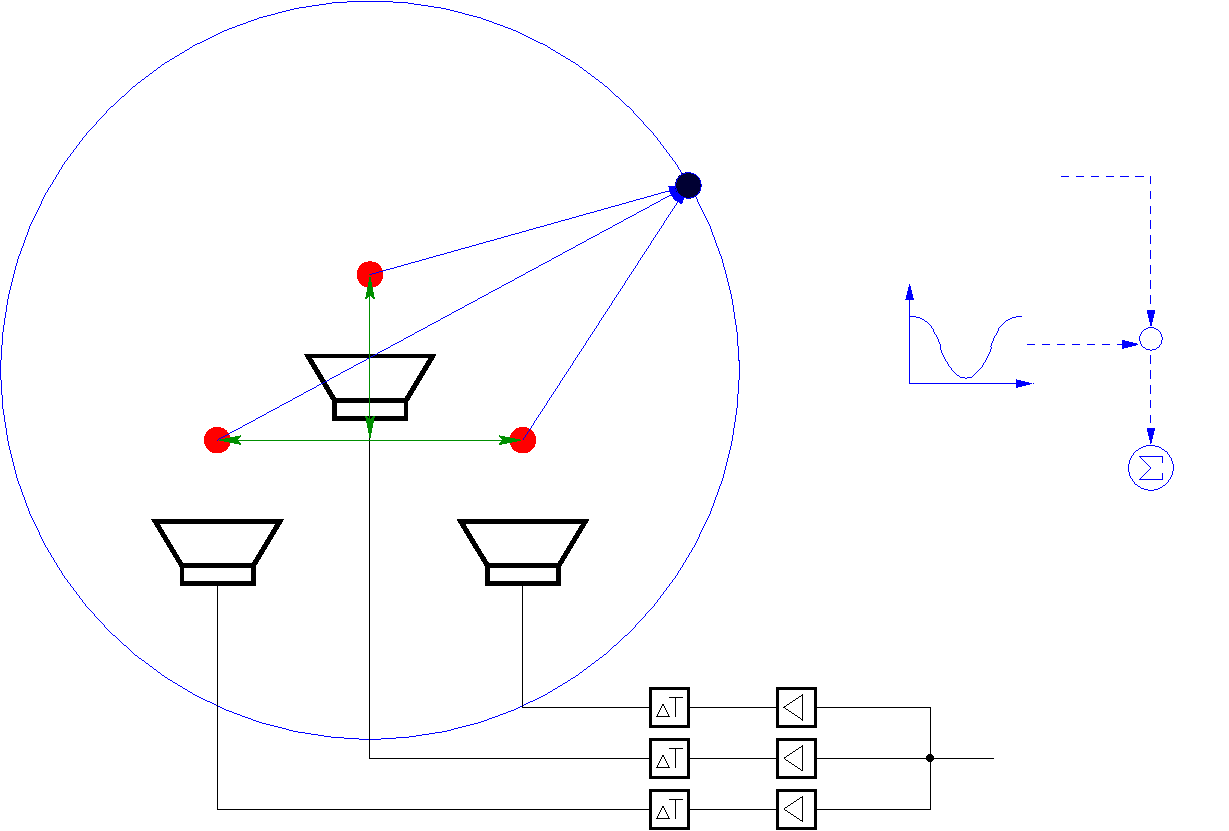
\includegraphics{genetic_setup_01.pdf}%
\end{picture}%
\setlength{\unitlength}{3937sp}%
\begingroup\makeatletter\ifx\SetFigFont\undefined%
\gdef\SetFigFont#1#2#3#4#5{%
  \reset@font\fontsize{#1}{#2pt}%
  \fontfamily{#3}\fontseries{#4}\fontshape{#5}%
  \selectfont}%
\fi\endgroup%
\begin{picture}(9844,6664)(-681,-4729)
\put(8509,-860){\makebox(0,0)[lb]{\smash{{\SetFigFont{20}{20.0}{\rmdefault}{\mddefault}{\updefault}{\color[rgb]{0,0,1}$\cdot$}%
}}}}
\put(2701,-1411){{\color[rgb]{0,0,0}Speaker A}%
}
\put(1441,-2761){{\color[rgb]{0,0,0}Speaker B}%
}
\put(3871,-2761){{\color[rgb]{0,0,0}Speaker C}%
}
\put(5941,-3661){{\color[rgb]{0,.56,0}\texttt{Va}}%
}
\put(5941,-4066){{\color[rgb]{0,.56,0}\texttt{Vb}}%
}
\put(5941,-4471){{\color[rgb]{0,.56,0}\texttt{Vb}}%
}
\put(4906,-4471){{\color[rgb]{0,.56,0}\texttt{Phic}}%
}
\put(4906,-4066){{\color[rgb]{0,.56,0}\texttt{Phib}}%
}
\put(4906,-3661){{\color[rgb]{0,.56,0}\texttt{Phia}}%
}
\put(2341,-601){{\color[rgb]{0,.56,0}\texttt{Ly}}%
}
\put(1081,-331){{\color[rgb]{1,0,0}Ac. Center A}%
}
\put(-179,-1681){{\color[rgb]{1,0,0}Ac. Center B}%
}
\put(3691,-1681){{\color[rgb]{1,0,0}Ac. Center C}%
}
\put(5131,659){{\color[rgb]{0,0,1}Pressure along the circumference}%
}
\put(5131,404){{\color[rgb]{0,0,1}of the array, calculated according}%
}
\put(5131,149){{\color[rgb]{0,0,1}to the augmented pressure equation \ref{eq:aug_omni}}%
}
\put(1801,-1771){{\color[rgb]{0,.56,0}\texttt{Lx}}%
}
\put(6436,-1366){{\color[rgb]{0,0,1}weighting curve}%
}
\put(8056,-2176){{\color[rgb]{0,0,1}fitness value}%
}
\end{picture}%
	\end{minipage}
	\end{sideways}
%\center
\caption{Phenotype and Genotype relations, visualization of genes and fitness evaluation. Alleles are denoted in \textcolor{green3}{green} and the fitness evaluation method is denoted in \textcolor{blue}{blue}.}
\label{fig:gene_setup}
\end{figure}
According to point  3. in \autoref{sec:ga_fundamental}, there needs to be a function that evaluates the fitness of every genotype based on some criteria. The way that this is achieved is also visualized in \autoref{fig:gene_setup}. The corresponding code is shown in Appendix \ref{axs:fitness}. The coordinates of a \textcolor{blue}{circle} around the centroid of the triangle between the \textcolor{red}{acoustic centers} are calculated. The position of the centroid will from now on be related to as the \textit{array center}. The radius of the \textcolor{blue}{circle} is significantly larger than the size of the speaker array. In this project, the chosen radius is \SI{10}{\meter} for both the analytical model and the simulation. From coordinates on the circumference, a set of coordinates, that describes the distance to each \textcolor{red}{acoustic center}, is deduced for each of the speakers. Using these coordinates, the gain and phase parameters from the alleles as well as the frequency, for which the optimization is excecuted, the pressure from each speaker is calculated using \autoref{eq:aug_omni}. The pressures are added in order to get the resulting pressure along the circumference. At this point it is crucial to take intro account the phase and therefore it is not the absolute pressure but the complex pressure that is summed.\\
The ultimate goal of running this \gls{ga} is getting a phenotype solution, that leads to particular desired directional characteristics of the speaker array. The desired characteristics are specified, by weighting the normed absolute pressure along the circumference according to some preference. This means, pressure in the direction in the direction, in which sound emission is desired, is assigned a low cost, whereas pressure in a direction, in which sound emission is undesired, is assigned a high cost. When the normed and weighted pressure is summed, a fitness value is calculated. The formerly described way of applying weight leads to lower values corresponding to fitter solutions.\\
The final point 4. from \autoref{sec:ga_fundamental} mentions probabilistic transition rules. The implementation of these is shown in Appendices \ref{axs:parents}, \ref{axs:offspring} and \ref{axs:mutation}. The genotypes, that are used to generate new genotypes for the subsequent generation are selected via tournament
selection \citep{tournament}. This ensures plenty of randomness while there is still some pressure caused by the fitness of the individual solution.
Offspring is then generated by combining the alleles of the parent genotype at a randomly determined ratio. This leads to two offspring genotypes with complementary ratios.
Furthermore there is a mutation function, that, with a comparatively low probability, changes one of the allele of any genotype to a randomly determined value.\\
A number of generations are computed after the initialization. The most fit genotype of the last generation that is computed should represent a near optimal solution to the beamforming problem. It has to be noted, that this routine has to be repeated for every frequency, for which a set of parameters is to be obtained.



\section{Inclusion of Prior Knowledge}\label{sec:ga_prior}
To simplify the optimization task, it is expedient to exploit knowledge and requirements given from the context of the project. This prior knowledge contains constraints that are given by practical issues. This leads to constraints, like the maximum distance between the acoustic centers, that is determined by the size of the anechoic chamber, in which the speaker array should be set up for measurements, or the minimum distance between the acoustic centers, which is determined by the physical size of the loudspeakers. It is possible to use the optimization to obtain parameters that lead to a main emission direction of the speaker array in any direction. However, for practical reasons the preferred solutions have either a single speaker on the line between the array center and main emission direction, or the connecting line between two acoustic centers perpendicularly to the formerly mentioned main emission direction. This leads to a symmetrical array configuration, which means, that optimal signal processing parameters are assumed to be equal for two of the three speakers. Implementing the \gls{ga} with this in mind, the optimization can be simplified.
Another form of prior knowledge is used when initializing the population. With trial-and-error style heuristics, some knowledge about the nature of fit solutions can be gained and implemented in the initialization function as an expectational value when setting up parameters as Gaussian random variables.\\
Prior knowledge is also incorporated in the way that the optimization is excecuted over the whole frequency range of \SIrange{60}{300}{\hertz}. Heuristic trials have shown, that the placement of the loudspeakers is much more critical for the optimization result at higher frequencies then it is at lower frequencies. When it is intended to actually set up a speaker array that is driven the signal processing parameters that are the result of the optimization process, and measure and experience the performance, then it is not feasible to have different speaker positions for different frequencies. For this reason it was initially planned to start the optimization process at the highest frequency. The speaker position would then be fixed. In the following optimization runs, only gain and phase are optimized. Using the population of the last generation from the previous frequency optimization, allows to have a smaller number of generations when optimizing for the adjacent frequency as some of the genotypes are already close to optimal. 
However, it has to be taken into account, that a comparison between the analytical model of the array and some \gls{fdtd}-simulation results is part of this project (see \autoref{sec:meas_vs_theory}). This leads to a discretization of the feasible values for the alleles \textcolor{green3}{\texttt{Lx}} and \textcolor{green3}{\texttt{Ly}}. This is not ideal for the implementation in this particular genetic algorithm. Additionally, the main axis response, as it is described in the next Section \ref{sec:main_axis}, leads to practical issues, where it is undesirable to apply significantly more voltage to speakers in at particular frequencies then at others. This has lead to the decision to fix the position according to a criterion related to the main axis response (see \autoref{ssec:cost_map}).


\section{Main axis response}\label{sec:main_axis}
\subsection{Analytical Considerations}\label{ssec:main_axis_formulas}
To assess the practicability of the speaker array, it can be investigated, how it behaves on the main axis, where the voluntary audience is assumed to be. In order to do this, the frequency dependent sound pressure level on the main axis $L_{p,beam}(f)$ is compared a reference pressure level $L_{p,ref}(f)$, that is emitted by three loudspeakers of the same kind as those in the array, placed closely together as illustrated in \autoref{fig:ref_omni_array}. These analytical considerations are undertaken using augmented omnidirectional sources (\autoref{eq:aug_omni}). The velocity for this reference sources is the same, as the one for two frontal sources of the array. In the reference case, all three sources are in phase.
We can introduce the frequency dependent beamforming cost $\Delta L_{p}(f)$ as the difference between the reference level $L_{p,ref}(f)$ and the beamformed level $L_{p,beam}(f)$ (see \autoref{eq:beam_cost}).  The beamformed level is a pressure level calculated similarly to the cost function in the optimization. The speakers are arranged triangularly and the velocity for speakers B and C is the same as in the formerly mentioned reference case, whereas the velocity and phase of speaker A are set according some optimization result. This case is illustrated in \autoref{fig:ref_caridioid_array}. For all calculations, a distance of $r\,=\,\SI{10}{\meter}$ will be used.
\begin{equation}\label{eq:beam_cost}
\Delta L_{p}(f)\,=\,L_{p,ref}(f)-L_{p,beam}(f)
\end{equation}

\begin{figure}[h]
	\centering
\begin{picture}(0,0)%
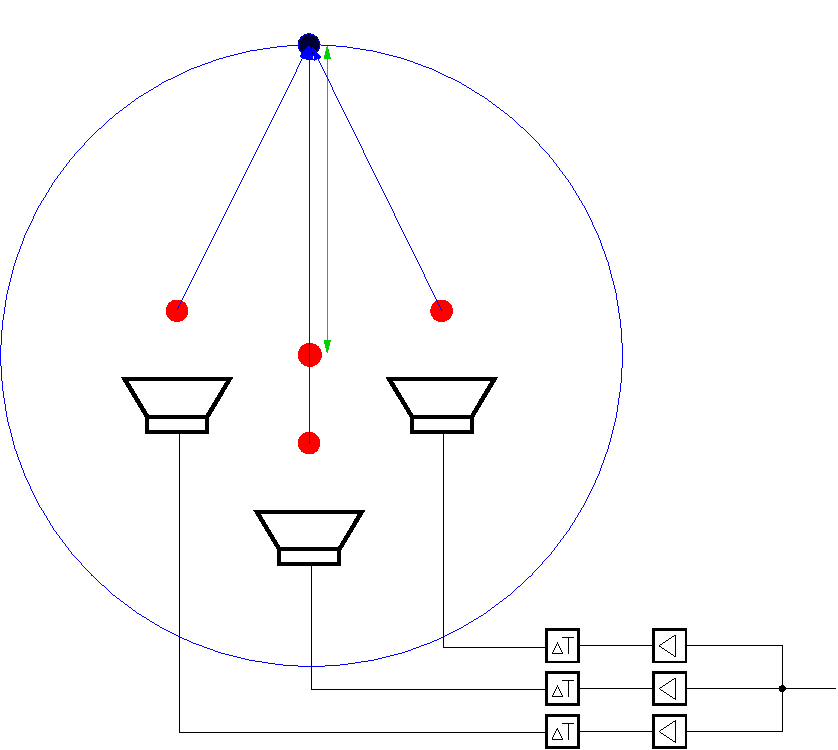
\includegraphics[scale=0.5]{ref_caridioid_array.pdf}%
\end{picture}%
\setlength{\unitlength}{1658sp}%
%
\begingroup\makeatletter\ifx\SetFigFont\undefined%
\gdef\SetFigFont#1#2#3#4#5{%
  \reset@font\fontsize{#1}{#2pt}%
  \fontfamily{#3}\fontseries{#4}\fontshape{#5}%
  \selectfont}%
\fi\endgroup%
\begin{picture}(7975,7142)(-672,-4729)
\put(5941,-3661){\color[rgb]{0,.56,0}\scriptsize{\texttt{Va}}}%
\put(5941,-4066){\color[rgb]{0,.56,0}\scriptsize{\texttt{Vb}}}%
\put(5941,-4471){\color[rgb]{0,.56,0}\scriptsize{\texttt{Vb}}}%
\put(4906,-4471){\color[rgb]{0,.56,0}\scriptsize{\texttt{Phib}}}%
\put(4906,-4066){\color[rgb]{0,.56,0}\scriptsize{\texttt{Phib}}}%
\put(4906,-3661){\color[rgb]{0,.56,0}\scriptsize{\texttt{Phia}}}%
\put(2271,2230){\color[rgb]{0,0,0}$L_{p,beam}$}%
\put(2535,219){\color[rgb]{0,.82,0}\SI{10}{\meter}}%
\put(2566,-1051){\color[rgb]{1,0,0}Array center}%
\put(2386,-3511){\color[rgb]{0,0,0}Speaker A}%
\put(1056,-2196){\color[rgb]{1,0,0}Ac. Center A}%
\put(-1150,-1051){\color[rgb]{1,0,0}Ac. Center B}%
\put(-1000,-2251){\color[rgb]{0,0,0}Speaker B}%
\put(3736,-601){\color[rgb]{1,0,0}Ac. Center C}%
\put(3646,-2251){\color[rgb]{0,0,0}Speaker C}%
\end{picture}%
	\caption{Configuration for main axis beamformed pressure.}
		\label{fig:ref_caridioid_array}
\end{figure}

\begin{figure}[h]
	\centering
\begin{picture}(0,0)%
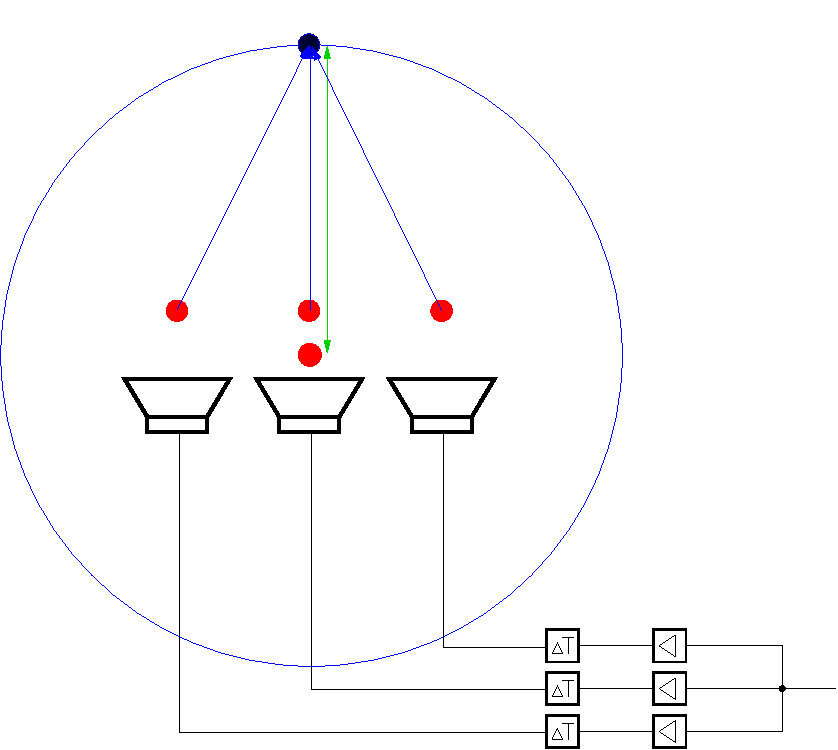
\includegraphics[scale=0.5]{ref_omni_array.pdf}%
\end{picture}%
\setlength{\unitlength}{1658sp}%3315sp}%
%
\begingroup\makeatletter\ifx\SetFigFont\undefined%
\gdef\SetFigFont#1#2#3#4#5{%
  \reset@font\fontsize{#1}{#2pt}%
  \fontfamily{#3}\fontseries{#4}\fontshape{#5}%
  \selectfont}%
\fi\endgroup%
\begin{picture}(7975,7142)(-672,-4729)
\put(1641,-201){\color[rgb]{1,0,0}Ac. Center A}%
\put(5941,-3661){\color[rgb]{0,.56,0}\texttt{Vb}}%
\put(5941,-4066){\color[rgb]{0,.56,0}\texttt{Vb}}%
\put(5941,-4471){\color[rgb]{0,.56,0}\texttt{Vb}}%
\put(4906,-4471){\color[rgb]{0,.56,0}\texttt{0}}%
\put(4906,-4066){\color[rgb]{0,.56,0}\texttt{0}}%
\put(4906,-3661){\color[rgb]{0,.56,0}\texttt{0}}%
\put(2271,2230){\color[rgb]{0,0,0}$L_{p,ref}$}%
\put(2535,219){\color[rgb]{0,.82,0}\SI{10}{\meter}}%
\put(-1409,-201){\color[rgb]{1,0,0}Ac. Center B}%
\put(3936,-651){\color[rgb]{1,0,0}Ac. Center C}%
\put(161,-2106){\color[rgb]{0,0,0}Speaker B}%
\put(1421,-2506){\color[rgb]{0,0,0}Speaker A}%
\put(2681,-2906){\color[rgb]{0,0,0}Speaker C}%
\put(2476,-1051){\color[rgb]{1,0,0}Former array center}%
\end{picture}%
	\caption{Configuration for reference pressure $L_{p,ref}$.}
		\label{fig:ref_omni_array}
\end{figure}
For practical applications, it is preferable to have the same frequency response from the speaker array on the main axis as for the case where no beamforming is executed. In order to achieve this, the input signal has to be sent through a filter with the same amplitude response as the beamforming cost. To avoid nonlinear behaviour from the loudspeakers, it is desirable to keep this equalization to a minimum. Because of this, another minimization criterion has emerged. It can be expressed mathematically as the integral over the beamforming cost.
\subsection{Signal Chain}\label{ssec:sig_chain}
The desired amplitude behaviour of the signals in the loudspeaker array can be achieved by using two filters. First, the signals to all three speakers is run through a filter, that is compensating the beamforming cost. This first filter only has to fulfill certain amplitude specifications, where phase does not matter. Secondly, the signal to the single speaker in the back of the array is run through another filter, that manipulates phase and amplitude according to specifications from \autoref{sec:opt_result} in order to make beamforming happen. The setup is illustrated in \autoref{fig:signal_setup}. Detailed information about the implementation of these filters will be given in \autoref{sec:filter_design}.
\begin{figure}[h]
	\centering
\begin{picture}(0,0)%
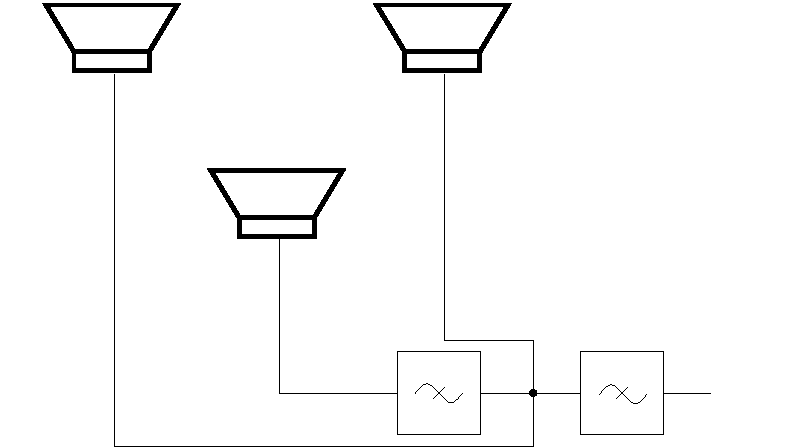
\includegraphics[scale=0.8]{filter_setup.pdf}%
\end{picture}%
\setlength{\unitlength}{3315sp}%4144sp}%
%
\begingroup\makeatletter\ifx\SetFigFont\undefined%
\gdef\SetFigFont#1#2#3#4#5{%
  \reset@font\fontsize{#1}{#2pt}%
  \fontfamily{#3}\fontseries{#4}\fontshape{#5}%
  \selectfont}%
\fi\endgroup%
\begin{picture}(6083,3409)(166,-4573)
\put(41,-1936){Speaker B}%

\put(3646,-1936){Speaker C}%

\put(2386,-3241){Speaker A}%

\put(5311,-4471){Cost Filter}%

\put(1286,-4471){Beamforming Filter}%

\end{picture}%
	\caption{Signal chain for beamforming.}
		\label{fig:signal_setup}
\end{figure}

%The following graph \autoref{fig:graph_plot_three_line} shows the absolute pressure from \SI{60}{\hertz} to \SI{300}{\hertz} of the aligned speaker model. 
%
%\begin{figure}[H]
%	\centering
%	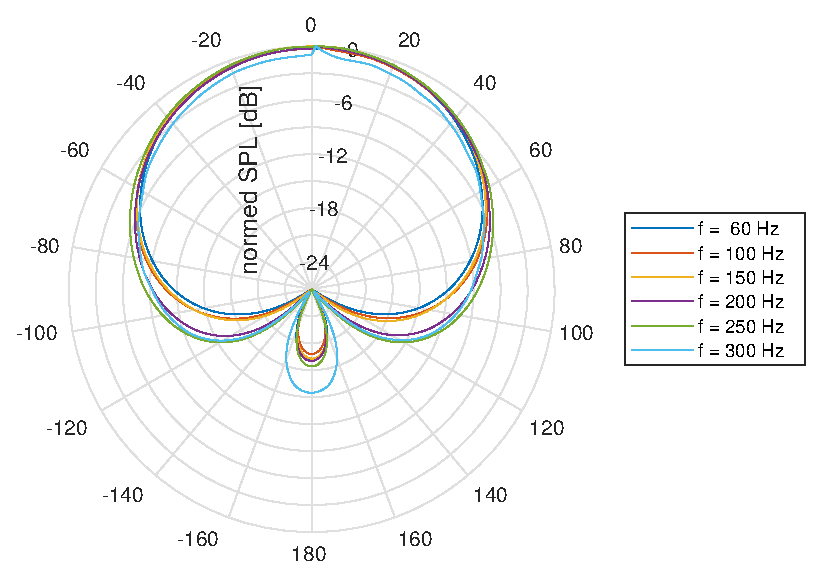
\includegraphics[width=0.7\textwidth]{expected_polar_pcor.eps}
%	\caption{The graph shows the frequency response of the aligned speaker model from \SI{60}{\hertz} to \SI{300}{\hertz}}
%		\label{fig:graph_plot_three_line}
%\end{figure}
\subsection{Settling on a position}\label{ssec:cost_map}
In order to make a a decision on the which parameters \textcolor{green3}{\texttt{Lx}} and \textcolor{green3}{\texttt{Ly}} will be used as fixed values for the final optimization process. The number of feasible solutions is limited by physical constraints when building a reasonable mounting contraption for the array and by the size of the speaker cabinets. It has therefore been decided to assess the beamforming cost via a brute force approach. The beamforming cost has been calculated for every combination of \textcolor{green3}{\texttt{Lx}} and \textcolor{green3}{\texttt{Ly}} in a \SI{5}{\centi\meter} grid. The absolute of the frequency dependent beamforming cost $\Delta L_{p}(f)$ has been intergrated numerically to result in a scalar value, referred to as the cost value. The lowest cost value corresponds to the most ``even" load on the speakers. The results are shown in \autoref{fig:cost_map}.
\begin{figure}[h]
	\centering
	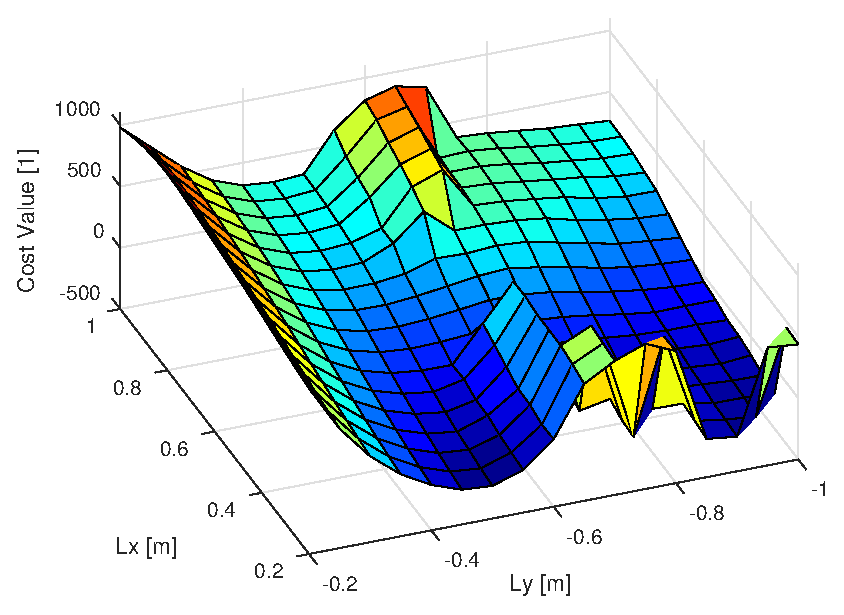
\includegraphics[width=0.7\textwidth]{cost_map.eps}
	\caption{Cost values for feasible acoustical center positions.}
		\label{fig:cost_map}
\end{figure}

\section{Optimization Results}\label{sec:opt_result}
The best genotypes for every frequency can be used to generate polar plots of the expected directional characteristics (\autoref{fig:opt_res_c}). Generating these is done similarly to the fitness evaluation by calculating the normed summed pressure along a circumference using \autoref{eq:aug_omni}.
Because the optimization algorithm has been fixed to a case, where the main axis of the array is orthogonal to the line between two of the acoustic centers, the signal for two of the speakers is the same. The relation between this signal and the signal for the remaining speaker can be plotted for phase and amplitude (\autoref{fig:opt_res_b}). The regressed curves can later be used to find filter parameter (see \autoref{sec:filter_design}).\\
Another plot of the expected directional characteristics is made, based on the regressed parameters, in order to estimate, which effect the filtering will have (\autoref{fig:opt_res_d}).
As mentioned before, in order to achieve this result, the speaker positions parameters \textcolor{green3}{\texttt{Lx}} and \textcolor{green3}{\texttt{Ly}} were fixed.  The beamforming cost is a frequency dependent value that is described in detail in \autoref{sec:main_axis}. For the given optimization, it is plotted in \autoref{fig:opt_res_a}. The results show, that in low frequencies the speaker array emits approx. \SI{6}{\decibel} less pressure than a comparable arrangement of speakers without beamforming. However, towards higher frequencies, the emitted pressure is higher, leading to negative cost values, with a peak around \SI{240}{\hertz} at approx. \SI{-2}{\decibel}. At frequencies higher than that, the graph tends to rise again and displays a value of approx. \SI{-1}{\decibel} at the upper frequency boundary of \SI{300}{\hertz}. It can be noted, that the values, that have been calculated with the augmented source model (\autoref{eq:aug_omni}) only diverge from those that have been calculated with perfectly omnidirectional sources by a negligible quantity.
In order to achieve compatibility with the \gls{fdtd} simulation (see \autoref{sec:fdtd_simulation}), the speaker positioning parameters have to fit within a \SI{5}{\centi\meter} grid. This lead to the decision to investigate the beamforming cost for different positions and to settle on a speaker positioning scheme based on the \SI{5}{\centi\meter}-discreteness and beamforming cost as well as practical considerations about the speaker placement.
\begin{figure}[H]
\begin{subfigure}[c]{0.5\textwidth}
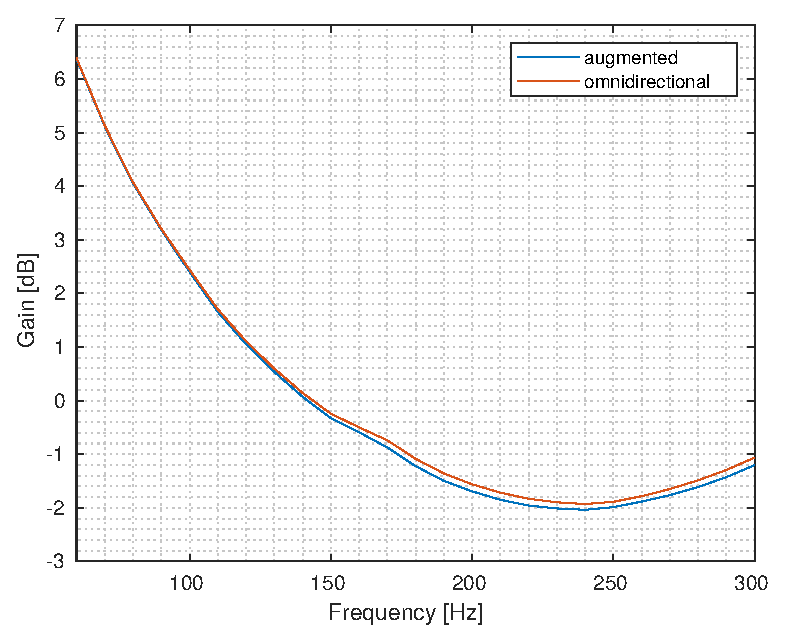
\includegraphics[width=0.85\textwidth]{opt_a.eps}
\subcaption{Beamforming cost}
\label{fig:opt_res_a}
\end{subfigure}
\begin{subfigure}[c]{0.5\textwidth}
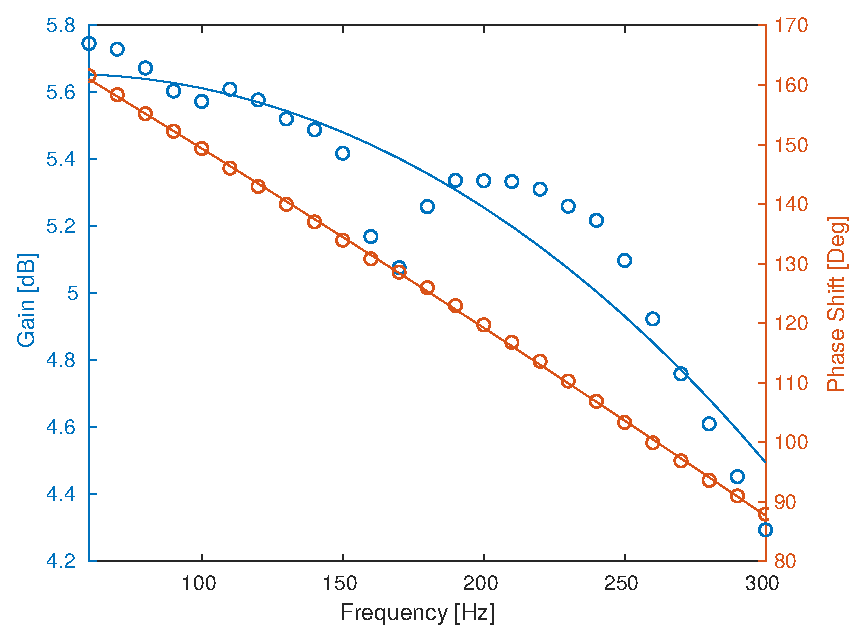
\includegraphics[width=0.95\textwidth]{opt_b.eps}
\subcaption{Beamforming filter requirements}
\label{fig:opt_res_b}
\end{subfigure}\\
\hspace{0.1\textheight}
\begin{subfigure}[c]{0.5\textwidth}
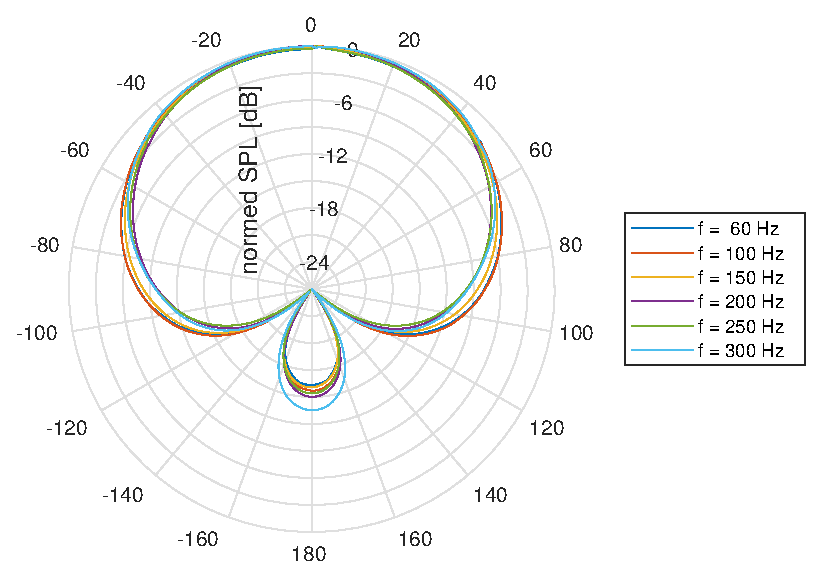
\includegraphics[width=0.95\textwidth]{opt_c.eps}
\subcaption{Directional characteristic, optimal, omnidirectional sources}
\label{fig:opt_res_c}
\end{subfigure}
\begin{subfigure}[c]{0.5\textwidth}
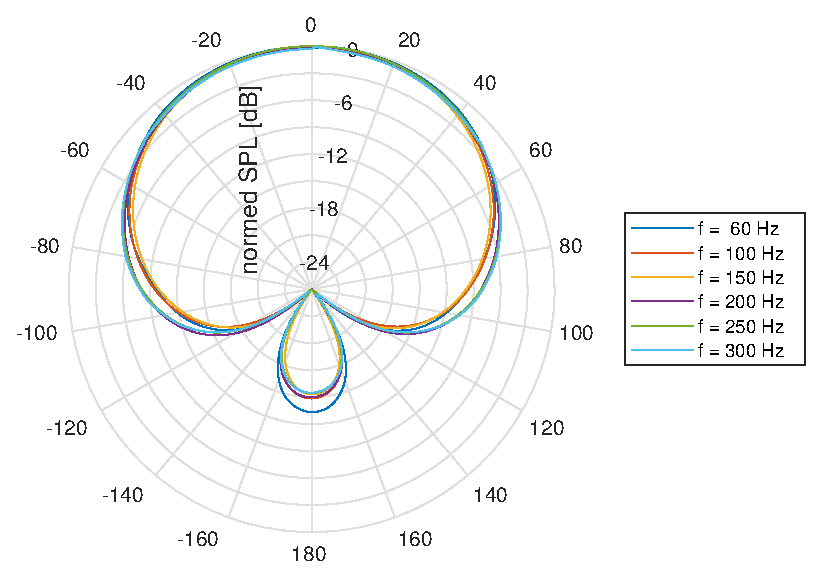
\includegraphics[width=0.95\textwidth]{polar_filtered.eps}
\subcaption{Directional characteristics, filtered, omnidirectional sources}
\label{fig:opt_res_d}
\end{subfigure}\\
\hspace{0.1\textheight}
%\begin{subfigure}[c]{0.5\textwidth}
%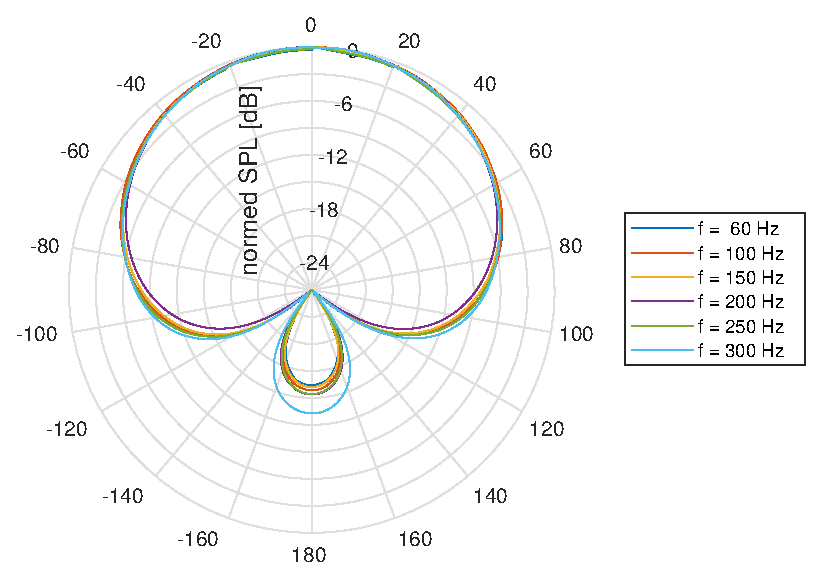
\includegraphics[width=0.95\textwidth]{opt_og_corrected.eps}
%\subcaption{Directional characteristics, optimal, pressure corrected sources}
%\label{fig:opt_res_d}
%\end{subfigure}
%\begin{subfigure}[c]{0.5\textwidth}
%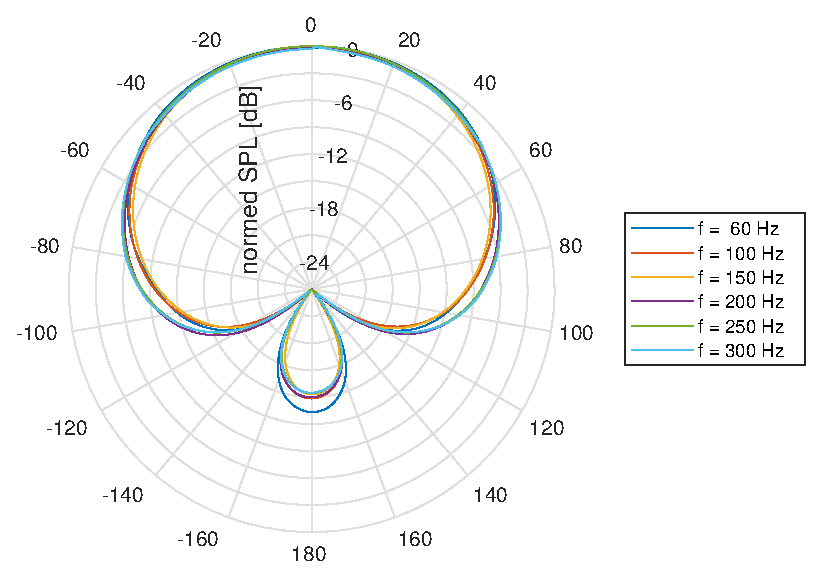
\includegraphics[width=0.95\textwidth]{opt_filter_corrected.eps}
%\subcaption{Directional characteristics, filtered, pressure corrected sources}
%\label{fig:opt_res_d}
%\end{subfigure}\\
\caption{Optimization results, pressure corrected cost function with correction table based on Appendix \ref{ax:directional_2}, \textcolor{green3}{\texttt{Lx}}\,$=$\,\SI{0.4}{\meter}, \textcolor{green3}{\texttt{Ly}}\,$=\,$\SI{-0.4}{\meter}}
		\label{fig:opt_res}
\end{figure}


\section{Conclusion on \gls{sp}-requirements}\label{sec:genetic_con}
The investigations have shown, that at least according to analytical descriptions, the directional characteristics of a triangular loudspeaker array can be shaped in a significant way. The positioning of loudspeakers plays an important role on the signal parameters, that are required. Changing the positions of the loudspeakers will lead to varying results in terms of beamforming cost and directional characteristics. While a main lobe in any direction in relation to the speaker array is technically possible, it has been decided to go with a simplified approach, where the main lobe of the array is perpendicular to a connecting line between two acoustic centers. This leads to a simplified scheme as illustrated in \autoref{fig:signal_setup}, where only two filters are required. The analytical estimates of the directional characteristics of the array will be compared to simulation results that will be obtained with \gls{fdtd} (see. \autoref{sec:fdtd_simulation}. Finally, an implementation of the filters will be executed and polar response measurements will be performed.